\documentclass[
    NAME={Dr. Helga Ingimundardóttir},
    EMAIL={helgaingim@hi.is},
    FACULTY={Iðnaðarverkfræðideild},
    TITLE={Spáum fyrir um framtíð gervigreindar},
    SUBTITLE={út frá akademísku sjónarmiði},
    SEMINAR={Stjórnvísi},
    DATE={22. febrúar 2025},
    WIDE=true,
    ICELANDIC=true
]{HI-LaTeX/hi-beamer}

\usepackage{pgfpages}
%\setbeameroption{show only notes}

\begin{document}
\note{
Grunnáherslur:
\begin{itemize}
    \item Áhrif á fræðasamfélagið.
    \item Hagnýtar tengingar við atvinnulíf og nýsköpun.
    \item Mikilvægi ábyrgðar og sjálfbærni.
\end{itemize}
}

\begin{frame}{Áhrif á háskólakennslu}
\begin{columns}
    \begin{column}{0.7\linewidth}
    \begin{block}{Nýjar áskoranir}
        \begin{itemize}
            \item ChatGPT og CoPilot breyta hvernig nemendur læra.
            \item Þörf fyrir gagnrýni á niðurstöður frá stórum módelum.
        \end{itemize}
    \end{block}
    \begin{block}{Tækifæri}
        \begin{itemize}
            \item Meiri áhersla á umfangsmeiri og flóknari verkefni.
            \item Stoðtæki gerir flóknar áskoranir leysanlegar fyrir nemendur.
        \end{itemize}
    \end{block}
    \note{
    ChatGPT breytir kennslu. Kennarar geta lagt meiri áherslu á gagnrýni og flóknari verkefni. Nemendur nýta stoðtækni til að læra dýpra.
    }        
    \end{column}
    \begin{column}{.2\linewidth}
        \centering
        
\includegraphics[width=\linewidth]{myndir/github-education.png}
    \end{column}
\end{columns}
\end{frame}

\begin{frame}{Gagnasiðfræði og ábyrg notkun}
\begin{columns}
    \begin{column}{0.7\linewidth}
    \begin{block}{Mikilvægi siðfræði}
        \begin{itemize}
            \item Siðferðileg notkun gervigreindar verður lykilatriði.
            \item Kennsla í gagnasiðfræði verður skylda.
        \end{itemize}
    \end{block}
    \begin{block}{EU AI Act}
        \begin{itemize}
            \item Áhersla á gagnsæi, ábyrgð og áhættumat.
            \item Alþjóðlegur staðall sem mun hafa áhrif á þróun gervigreindar.
        \end{itemize}
    \end{block}
    \note{
    Siðferðileg notkun gervigreindar verður mikilvægari. EU AI Act setur skýra ramma um ábyrgð og gagnsæi.

    EU AI Act er regluverk Evrópusambandsins sem tryggir örugga, gagnsæja og siðferðilega notkun gervigreindar með áherslu á áhættumat og ábyrgð.

    Við kennum gagnasiðfræði sem hluta af valáfanga í iðnaðarverkfræði, kennt af Henry Alexander Henrysson við Siðfræðistofnun HÍ, en í ljósi hversu mikilvægt þetta er fyrir framtíðina ætlum við að færa þessa lotu inn í skyldunámskeið, og hvetja aðrar verkfræðideildir til að láta sína nemendur taka gagnasiðfræði líka.
    }
    \end{column}
    \begin{column}{.2\linewidth}
        \centering
        
\includegraphics[width=\linewidth]{myndir/eu-ai-act.png}
    \end{column}
\end{columns}
\end{frame}

\begin{frame}{Sjálfbærni og hagkvæmni}
\begin{columns}
    \begin{column}{.4\linewidth}
        \centering
        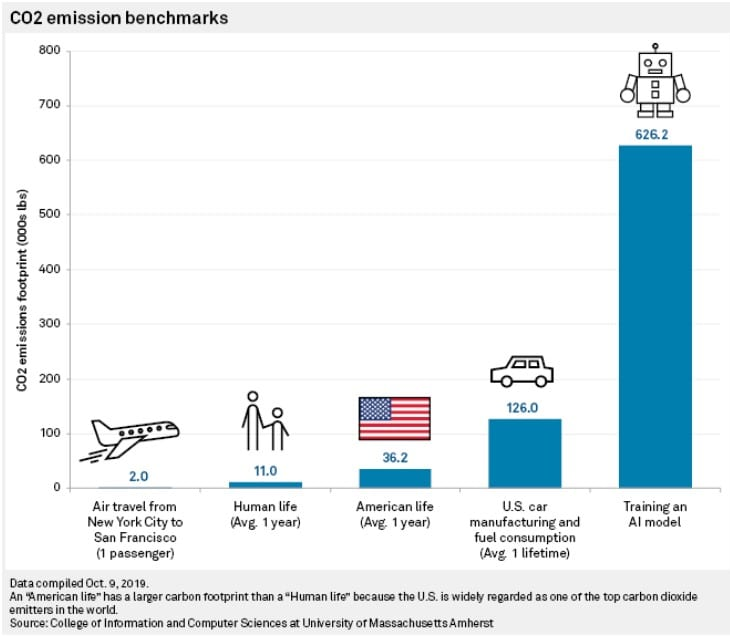
\includegraphics[width=\linewidth]{myndir/co2-emission.jpg}
    \end{column}
    \begin{column}{0.58\linewidth}
    \begin{block}{Áskoranir}
        \begin{itemize}
            \item Keyrsla stórra gervigreindalíkana krefst mikils reikniafls og orku.
            \item Loftslagsáhrif og kostnaður eru veruleg vandamál.
        \end{itemize}
    \end{block}
    \begin{block}{Lausnir}
        \begin{itemize}
            \item Nota innlent reikniafl á grænum orkugjöfum.
            \item \emph{DeepSeek} í Kína þjálfaði módel á brotabroti kostnaðarins með hagkvæmni í forgrunni.
        \end{itemize}
    \end{block}
    \note{
    Sjálfbærni er lykilatriði. Með nýrri tækni má draga úr kostnaði og umhverfisáhrifum. DeepSeek er gott dæmi um hagkvæma nálgun.

    DeepSeek, kínverskt gervigreindarfyrirtæki, kynnti nýlega DeepSeek V3, stórt mállíkan fyrir chat-bot með 600 milljarða vigra, þjálfað á 14,8 trilljónum tákna. Þjálfunarkostnaður þess var undir 6 milljónum Bandaríkjadala, sem er mun lægra en þjálfunarkostnaður GPT-4 frá OpenAI, sem var um 78 milljónir dala. 
    }
   \end{column}
\end{columns}
\end{frame}

\begin{frame}{Réttlæti í gervigreindarmódelum}
\begin{columns}
    \begin{column}{.25\linewidth}
        \centering
        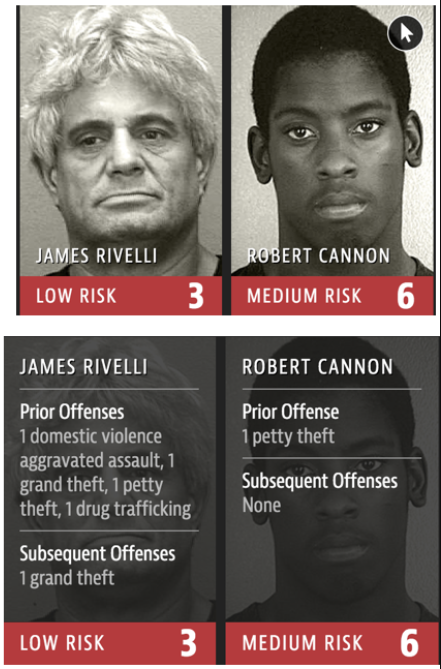
\includegraphics[width=\linewidth]{myndir/ai-bias.png}
    \end{column}
    \begin{column}{0.6\linewidth}
    \begin{block}{Áhrif gagna}
        \begin{itemize}
            \item Gögnin móta niðurstöður módela – þau þurfa að vera fjölbreytt og sanngjörn.
        \end{itemize}
    \end{block}
    \begin{block}{Markmið}
        \begin{itemize}
            \item Sanngirni í gagnasöfnun og \emph{markföllum}.
            \item Sanngirni sem lykilatriði frá upphafi líkangerðar.
        \end{itemize}
    \end{block}
    \note{
    Gögn þurfa að vera fjölbreytt og sanngjörn. Sanngirni í þróun módela skiptir lykilmáli til að byggja traust.
    }
\end{column}
\end{columns}
\end{frame}

\begin{frame}{ArtInRare: Gervigreind og listir}
    \begin{block}{Um verkefnið}
        \begin{itemize}
            \item Samevrópskt rannsóknarverkefni sem hófst haustið 2024.
            \item Markmið: Samtvinnun gervigreindar og listrannsókna á siðferðilegan hátt.
            \item Stendur yfir til haustið 2028.
        \end{itemize}
    \end{block}
    \begin{block}{Viðfangsefni}
        \begin{itemize}
            \item Siðferðileg nálgun á notkun gervigreindar í listum.
            \item Hvernig má efla sköpunarferlið með nýsköpun í gervigreind.
            \item Áhersla á samstarf milli fræðigreina og listafólks.
        \end{itemize}
    \end{block}
    \note{
    Artistic Intelligence - Responsiveness, accessibility, responsibility, equity (ARTinRARE) er samevrópskt verkefni sem miðar að því að styðja við listamenn og rannsakendur. 
    Verkefnið leggur áherslu á að þróa gervigreind sem stuðlar að nýsköpun án þess að skerða réttindi eða sjálfstæði listafólks. 
    Það sýnir hvernig gervigreind getur orðið hluti af skapandi ferli.
    }
\end{frame}


\begin{frame}{Ólíkar tegundir gervigreindar}
Gervigreind er ekki aðeins \emph{spunagreind}...
    \begin{figure}
        \centering
        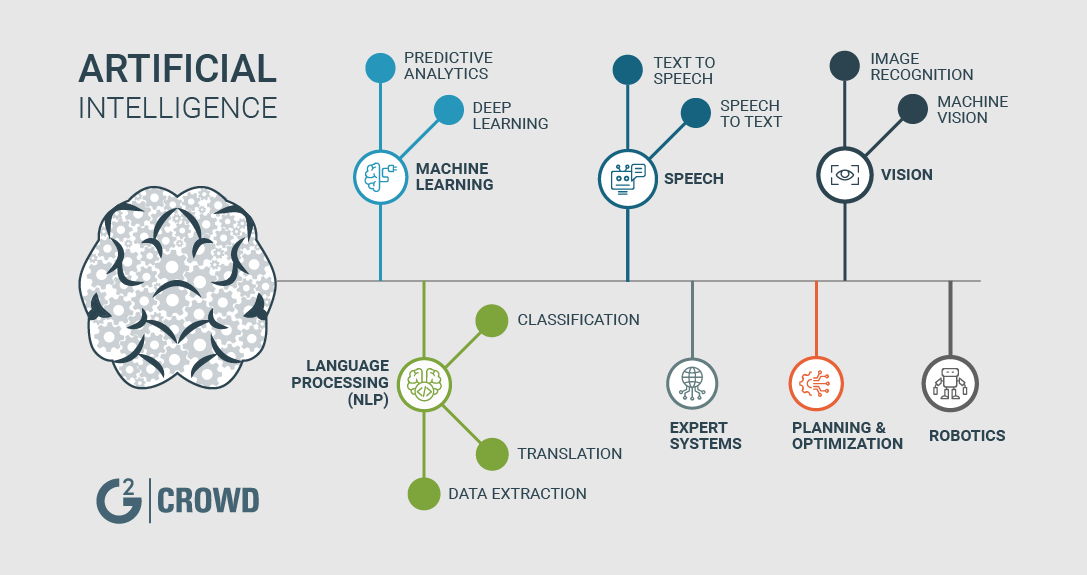
\includegraphics[width=.8\linewidth]{myndir/ai-types.png}
    \end{figure}
\end{frame}


\begin{frame}{Spurningar?}
    \begin{columns}        
        \begin{column}{0.5\textwidth} 
        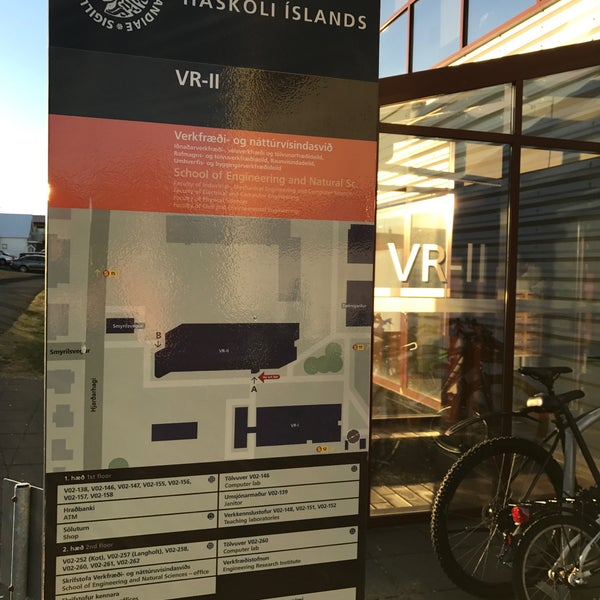
\includegraphics[height=\textwidth]{myndir/vr2.jpg}
        \end{column}
        \hfill
        \begin{column}{0.4\textwidth} 
        
            \begin{alertblock}{Hafið samband}
            \begin{description}
                \item[Aðsetur] VR-II, Háskóli Íslands
                \item[Sími] 525-4630
                \item[Netfang] helgaingim@hi.is
            \end{description}
            \end{alertblock}
        \end{column}
    \end{columns}    
\end{frame}

\end{document}